\documentclass[a4paper,12pt]{article}
\usepackage{graphicx}
\usepackage{hyperref}
\usepackage{titlesec}
\usepackage{booktabs}
\usepackage{float}
\usepackage{xcolor}
\usepackage{mathptmx}  % Times New Roman-like font
%\usepackage[backend=biber]{biblatex}



\title{\textbf{Speech Understanding}\\
\bigskip
\bigskip
\bigskip
{Programming Assignment-1}\\
\bigskip\bigskip\bigskip
{Project Report - Q-2-Task B} 
\bigskip\bigskip\bigskip\\
    {Comparative Analysis of \\Spectrograms Across Music Genres}
}
\bigskip\bigskip\bigskip

\author{\textbf{Prepared By:}\\Shyam Vyas (M23CSA545)}

\begin{document}
\maketitle

\newpage
\tableofcontents
\newpage

\newpage
\section{Introduction}
The spectrogram is a powerful tool for analyzing audio signals, providing a visual representation of frequency content over time. Different music genres exhibit unique spectral characteristics due to variations in instrumentation, rhythm, and production techniques. This report compares spectrograms of four songs from distinct genres—Rock, Classical, Jazz, and Electronic—to identify genre-specific spectral patterns and analyze their auditory structures.
\newpage
\section{Methodology}

\subsection{Selection of Songs}
The following songs were selected for analysis, representing a diverse range of musical styles:
\begin{itemize}
\item \textbf{Rock:} "I Have a Rock Soul" – A high-energy rock anthem featuring powerful guitar riffs and dynamic vocals.
\item \textbf{Classical:} "Simasx27s Songs Classical" – A beautifully composed orchestral piece with intricate melodies and rich harmonies.
\item \textbf{Jazz:} "Havana Beach Club Pop" – A smooth and lively jazz track with expressive saxophone solos and a rhythmic groove.
\item    \textbf{Electronic:} "Hip Pop Vol 6" – A pulsating electronic composition with deep basslines, layered synths, and an engaging beat.
\end{itemize}


\subsection{Preprocessing}
\begin{itemize}
    \item Each song was converted to WAV format and standardized to a sampling rate of 22050 Hz for consistency.
\item The audio was processed using Short-Time Fourier Transform (STFT) with a Hann window to reduce spectral leakage and improve frequency resolution.
\item A window size of 2048 samples was used, and the STFT magnitude was converted to decibels for visualization.
\end{itemize}

\subsection{Spectrogram Generation}
\begin{itemize}
\item Librosa and Matplotlib were used to compute and visualize spectrograms.
\item The time (x-axis) and frequency (y-axis) components were analyzed to observe the distribution of energy across different frequencies..
\end{itemize}
\newpage
\section{Spectrogram Analysis}
\subsection{Rock ("I Have a Rock Soul")}
\begin{itemize}
\item The spectrogram shows a broad frequency range, with significant energy in the mid and high frequencies, corresponding to electric guitars and vocals.
\item Percussion elements (e.g., drums) appear as transient bursts of energy in the low-frequency range.
\item Dynamic variations due to shifts in instrumentation are clearly visible.
\begin{figure}[H]
    \centering
    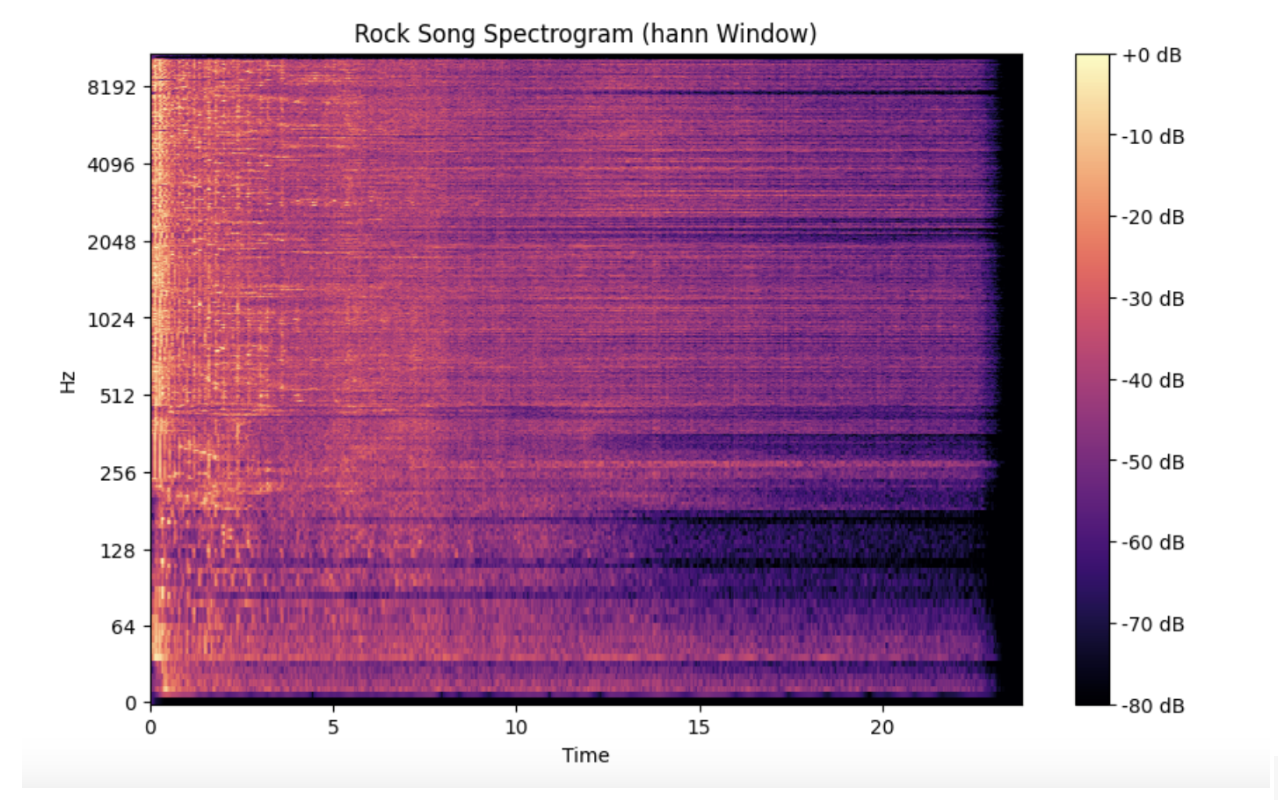
\includegraphics[width=1\linewidth]{RockSG.png}
    \caption{Rock Song Spectrogram (hann window)}
    \label{fig:enter-label}
\end{figure}
\end{itemize}
\newpage
\subsection{Classical ("Simasx27s Songs Classical")}
\begin{itemize}
\item The spectrogram primarily contains smooth harmonic structures in the mid-frequency range, corresponding to orchestral notes.
\item Unlike Rock, there are no sudden transient bursts, reflecting the continuous nature of classical compositions.
\item   Energy is distributed over longer durations, emphasizing sustained notes rather than rhythmic beats.
\begin{figure}[H]
    \centering
    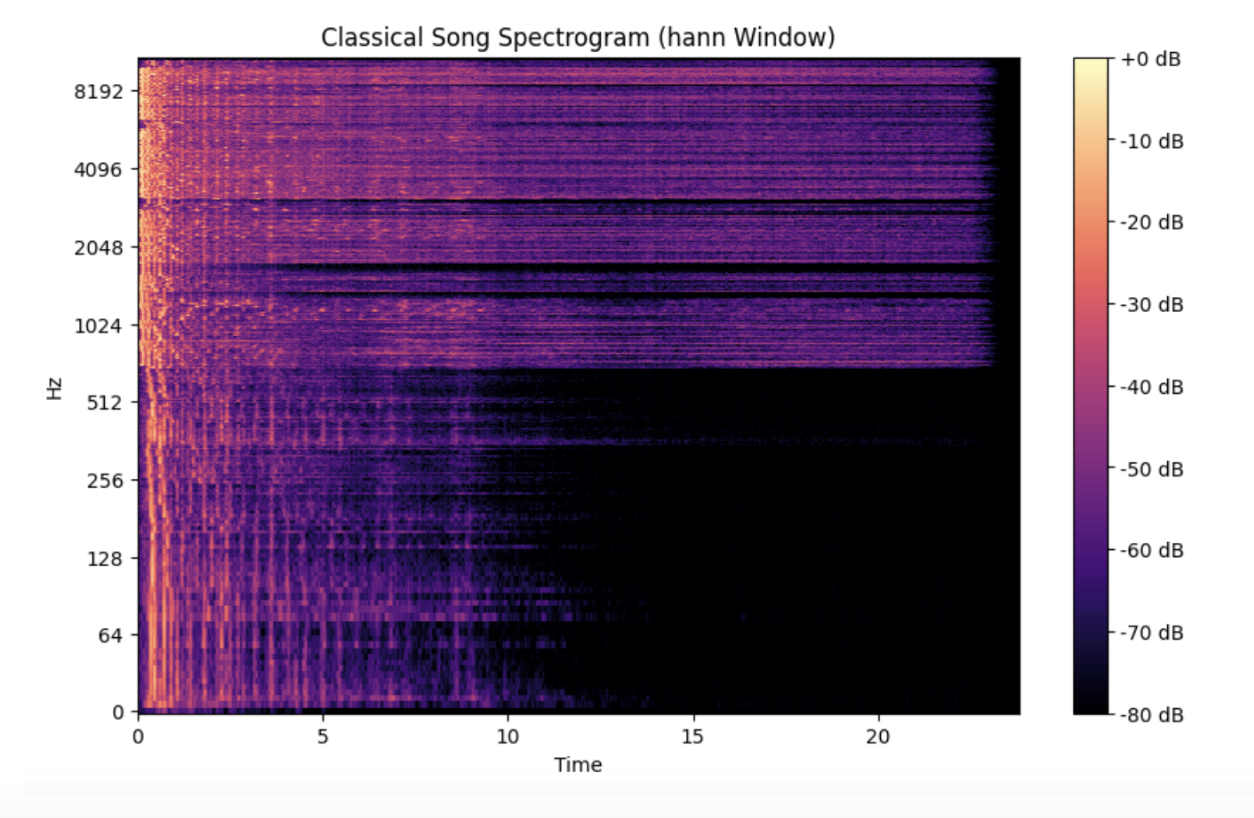
\includegraphics[width=1\linewidth]{ClassicalSPG.png}
    \caption{Classical Song Spectrogram (hann window)}
    \label{fig:enter-label}
\end{figure}
\end{itemize}
\newpage
\subsection{Jazz ("Havana Beach Club Pop")}
\begin{itemize}
\item The spectrogram displays rhythmic complexity, with frequent note changes and variations in intensity.
\item The double bass and drum set create periodic low-frequency pulses, while the saxophone and piano contribute energy to the mid-high frequency range.
\item Spectral patterns show improvisational variations, with unpredictable shifts in energy distribution.
\begin{figure}[H]
    \centering
    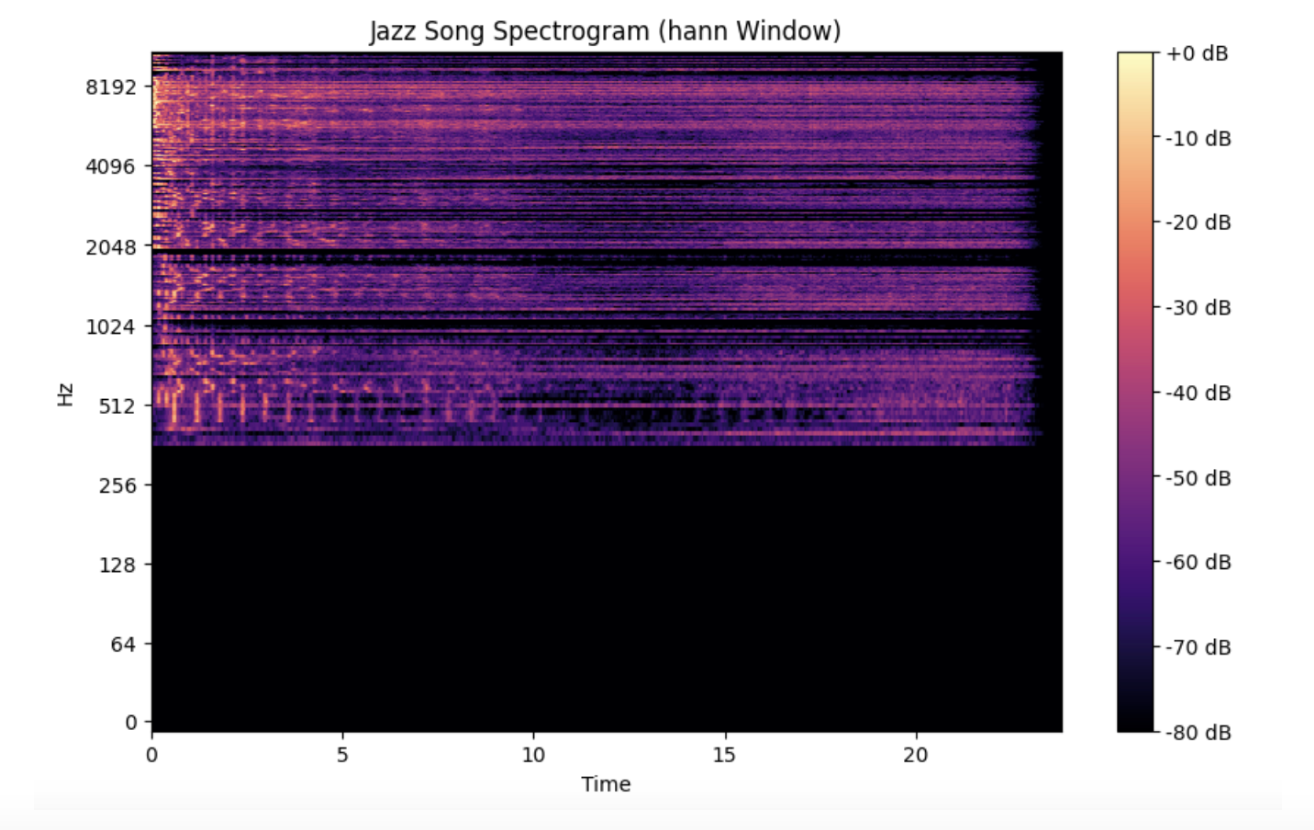
\includegraphics[width=1\linewidth]{JazzSongSPGM.png}
    \caption{Jazz Song Spectrogram (hann window)}
    \label{fig:enter-label}
\end{figure}
\end{itemize}
\newpage
\subsection{Electronic ("Hip Pop Vol 6)}
\begin{itemize}
\item The spectrogram reveals a consistent low-frequency presence, characteristic of electronic music’s heavy bass.
\item Higher frequencies exhibit repetitive patterns, reflecting looped synthesizers and digitally produced sounds.
\item Unlike Jazz, Electronic music shows a more structured, loop-based pattern with periodic energy peaks.
\begin{figure}[H]
    \centering
    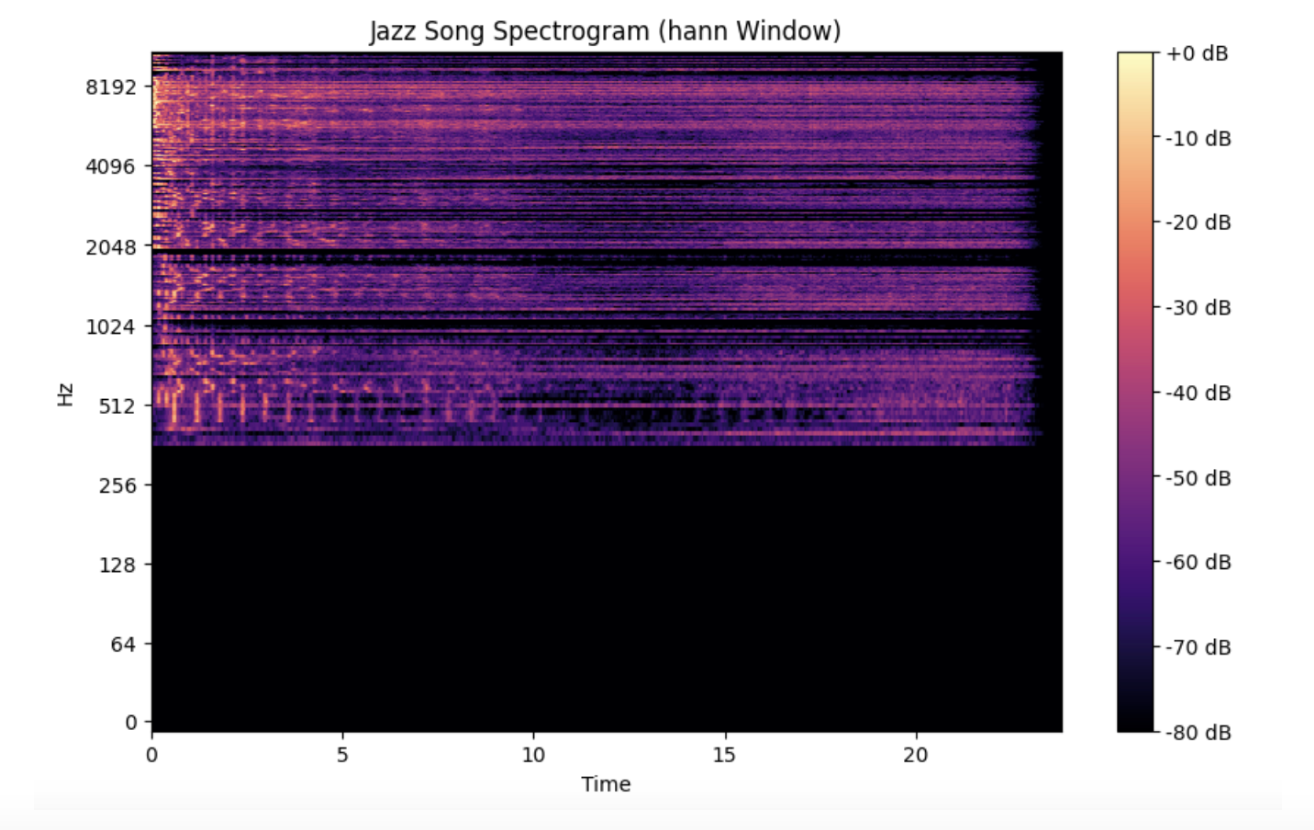
\includegraphics[width=1\linewidth]{ElectronicSongSPG.png}
    \caption{Electronic Song Spectrogram (hann window)}
    \label{fig:enter-label}
\end{figure}
\end{itemize}

\newpage
\section{Comparative Analysis}
\begin{itemize}
\item Rock and Jazz exhibit complex harmonic structures with rhythmic variations, but Jazz has more improvisational energy shifts.
\item Classical music has smooth transitions and sustained notes, while Electronic music is highly repetitive with strong bass presence.
\item Electronic and Rock music share high-energy peaks, but Rock features natural instrument sounds, whereas Electronic is synthetically generated.

\begin{figure}[H]
    \centering
    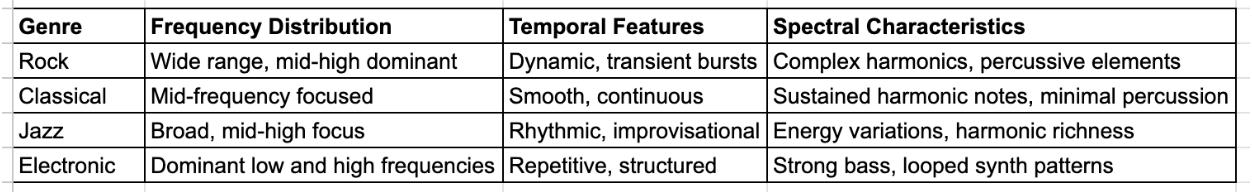
\includegraphics[width=1\linewidth]{ComparativeStudy.png}
    %\caption{Comparative }
    \label{fig:enter-label}
\end{figure}
\end{itemize}

\newpage
\section{Conclusion}
The spectrogram analysis highlights the distinct genre-based characteristics in frequency distribution, rhythm, and spectral energy. Classical music exhibits smooth harmonics, Rock and Jazz have complex spectral variations, and Electronic music is structured with strong bass elements. Understanding these patterns can aid in genre classification and audio signal processing applications. Future work could explore deep learning-based genre classification using spectrogram features.


\newpage
\section{Code Repository}
\href{https://github.com/IITJ-Projects/M23CSA545_PA1.git}{ GitHub Repository}
\addcontentsline{toc}{section}{References}
%\addbibresource{references.bib}
%\printbibliography[heading=bibintoc, title={References}]
\begin{thebibliography}{9}
    \bibitem{example} \href{https://www.kaggle.com/code/sujaykapadnis/audio-machine-learning-for-speech-recog-intro}{Audio Machine Learning for speech Recog Intro}
    \bibitem{example2} \href{https://www.kaggle.com/code/jerrypeng/dsp-tutorial-3-demos-for-speech-processing}{DSP Tutorial 3: Demos for speech processing}
    \bibitem{example3} \href{https://www.kaggle.com/code/santoshkumar/understanding-audio-data-getting-started}{Understanding-audio-data[getting-started]}
     \bibitem{documentation} \href{https://www.overleaf.com/}{ Latex Documentation - Overleaf}
\end{thebibliography}

\end{document}
